\documentclass{article}

%------------------------- Carga de paquetes ---------------------------
%
% Si no necesitás algún paquete, comentalo.
%

%
% Definición del tamaño de página y los márgenes:
%
\usepackage[a4paper,headheight=16pt,
            top=2.0cm,
            bottom=2.0cm,
            left=1.8cm,
            right=1.8cm]{geometry}

%\usepackage{caption}
%\usepackage{subcaption}

\usepackage{float}

\usepackage{wrapfig}

%
% Vamos a escribir en castellano:
%
\usepackage[spanish]{babel}
\usepackage[utf8]{inputenc}

\usepackage{adjustbox}

%\usepackage{pythontex}
\usepackage{pdfpages}
\usepackage{circuitikz}

\usepackage{multicol}

\usepackage{multirow}

%\usepackage{apacite} % O apacite si no lo tienes instalado, o natbib con opciones APA
%\usepackage{url}
%\bibliographystyle{apacite}
%\bibliography{refs}

%
% Si preferís el tipo de letra Helvetica (Arial), descomentá las siguientes
% dos lineas (las fórmulas seguirán estando en Times):
%
%\usepackage{helvet}
%\renewcommand\familydefault{\sfdefault}

%
% El paquete amsmath agrega algunas funcionalidades extra a las fórmulas. 
% Además defino la numeración de las tablas y figuras al estilo "Figura 2.3", 
% en lugar de "Figura 7". (Por lo tanto, aunque no uses fórmulas, si querés
% este tipo de numeración dejá el paquete amsmath descomentado).
%
\usepackage{amsmath}
\usepackage{amssymb}

%
% Para tener cabecera y pie de página con un estilo personalizado:
%
\usepackage{fancyhdr}

% Graficos
\usepackage{graphicx}

%Hipervinculos
\usepackage{hyperref}
\hypersetup{
    colorlinks=true,
    linkcolor=black,
    filecolor=magenta,      
    urlcolor=cyan
    }
%
% Para poner el texto "Figura X" en negrita:
% (Si no tenés el paquete 'caption2', probá con 'caption').
%
\usepackage[hang,bf]{caption}

% Para enumerar con letras
\usepackage[shortlabels]{enumitem}

% Para unidades
\usepackage{siunitx}
\DeclareSIUnit\division{div}
\sisetup{output-decimal-marker = {,}}

%
% Todas las imágenes están en el directorio includes:
%
\newcommand{\imgdir}{includes}
\graphicspath{{\imgdir/}}

\usepackage[capitalize, nameinlink, spanish]{cleveref}


\usepackage{listings}
\usepackage{xcolor}

\definecolor{codegreen}{rgb}{0,0.6,0}
\definecolor{codegray}{rgb}{0.5,0.5,0.5}
\definecolor{codepurple}{rgb}{0.58,0,0.82}
\definecolor{backcolour}{rgb}{0.95,0.95,0.92}

\lstdefinestyle{mystyle}{
	backgroundcolor=\color{backcolour},   
	commentstyle=\color{codegreen},
	keywordstyle=\color{magenta},
	numberstyle=\tiny\color{codegray},
	stringstyle=\color{codepurple},
	basicstyle=\ttfamily\footnotesize,
	breakatwhitespace=false,         
	breaklines=true,                 
	captionpos=b,                    
	keepspaces=true,                 
	numbers=left,                    
	numbersep=5pt,                  
	showspaces=false,                
	showstringspaces=false,
	showtabs=false,                  
	tabsize=2
}

\lstset{style=mystyle}
\usepackage{float}

\usepackage[indent]{parskip}

\usepackage{textcomp}
\usepackage{gensymb}




\begin{document}

    \renewcommand{\listtablename}{Índice de tablas}
    \renewcommand{\tablename}{Tabla}

    
	
	%
	% Hago que en la cabecera de página se muestre a la derecha la sección,
	% y en el pie, en número de página a la derecha:
	%
	\pagestyle{fancy}
	\renewcommand{\sectionmark}[1]{\markboth{}{\thesection\ \ #1}}
	\lhead{}
	\chead{}
	\rhead{\rightmark}
	\lfoot{}
	\cfoot{}
	\rfoot{\thepage}


\pagenumbering{arabic}
\thispagestyle{empty}

\begin{titlepage}
    \centering
    
    % Logo
    \vspace*{1.5cm}
    
\includegraphics[width=3.5cm]{fiuba.pdf}
    
    \vspace{1.5cm}
    
    % Universidad
    \Large\textsc{Universidad de Buenos Aires}\\
    \Large\textsc{Facultad de Ingeniería}
    
    \vspace{1cm}
    
    \large\textsc{Tesis}
    
    \vfill
    
    % Título
    {\Huge\bfseries
        QCM
    }
    
    \vfill
    
    % Fecha
    \large Mayo 2026
    
    \vspace{1.5cm}
    
    % Datos del alumno
    \begin{tabular}{rl}
        \textbf{Alumno:} & Aguirre Walter Mario \\
        \textbf{Padrón:} & 106328 \\
        \textbf{Correo:} & waguirre@fi.uba.ar \\
    \end{tabular}
    
    \vspace*{1cm}
    
\end{titlepage}


\tableofcontents
 
\newpage


\section{Introducción}

Las películas delgadas desempeñan un papel fundamental en diversas áreas de la ingeniería y la ciencia de materiales, especialmente en aplicaciones que requieren un control preciso de las propiedades físicas de los materiales en escalas micrométricas y nanométricas. Su utilización abarca campos como la microelectrónica, los sensores y los recubrimientos funcionales, entre otros. En este contexto, el control de los parámetros asociados al proceso de fabricación resulta determinante para garantizar la reproducibilidad y las características finales de las películas obtenidas.

Entre las distintas técnicas empleadas para la fabricación de películas delgadas se encuentra la ablación láser pulsada (\textit{Pulsed Laser Deposition}, PLD), una técnica de deposición física en fase vapor que permite transferir material desde un blanco hacia un sustrato mediante la interacción con pulsos láser de alta energía. Durante este tipo de procesos, la medición del espesor depositado constituye una variable de particular interés, ya que permite caracterizar y controlar el crecimiento de la película durante la deposición.

Una de las técnicas ampliamente utilizadas para este propósito es la microbalanza de cristal de cuarzo (\textit{Quartz Crystal Microbalance}, QCM). Su principio de funcionamiento se basa en la variación de la frecuencia de resonancia de un cristal piezoeléctrico de cuarzo ante cambios de masa sobre su superficie. Bajo determinadas condiciones de operación, esta variación puede relacionarse con la masa depositada por unidad de área mediante la ecuación de Sauerbrey y, conociendo las propiedades del material depositado, utilizarse posteriormente para estimar el espesor de la película. De esta manera, una QCM permite realizar un seguimiento \textit{in situ} del proceso de deposición a partir de la medición precisa de pequeñas variaciones en la frecuencia de resonancia del cristal.

Los sistemas comerciales destinados al monitoreo de espesor mediante QCM ofrecen soluciones de elevada precisión y estabilidad. Sin embargo, su costo puede representar una limitación para laboratorios de investigación y desarrollos experimentales con recursos acotados. Esto motiva el desarrollo de alternativas basadas en componentes electrónicos de propósito general y sistemas embebidos que permitan implementar las funciones fundamentales de estos instrumentos con un costo considerablemente menor.

En este marco, el presente trabajo propone el diseño, implementación y caracterización de un sistema de monitoreo de espesor de películas delgadas basado en una microbalanza de cristal de cuarzo y electrónica embebida. El sistema está orientado a su integración con una cámara de PLD y tiene como objetivo realizar la adquisición y el procesamiento de la frecuencia de resonancia del cristal en tiempo real, permitiendo relacionar sus variaciones con la masa y el espesor del material depositado.

El desarrollo comprende el diseño y caracterización de la electrónica asociada a la excitación del cristal de cuarzo, la implementación de un sistema para la medición precisa de su frecuencia de oscilación y el desarrollo de las herramientas necesarias para la adquisición, procesamiento y visualización de los datos. Se busca así obtener una plataforma de bajo costo, modular y adaptable que pueda ser utilizada para el monitoreo experimental de procesos de deposición de películas delgadas mediante PLD.


\section{Diseño del circuito oscilador}
\label{sec:oscilador}

Para realizar la medición de las variaciones de frecuencia del cristal de cuarzo es necesario incorporarlo a un circuito capaz de mantenerlo en oscilación. La frecuencia de la señal generada puede ser posteriormente adquirida mediante un sistema de conteo y utilizada para determinar los cambios producidos por la deposición de masa sobre la superficie del cristal.

\subsection{Oscilador basado en inversor lógico}
\label{subsec:oscilador_pierce}

El circuito implementado se basa en una configuración de oscilador tipo Pierce utilizando un inversor lógico 74HC04 como elemento activo. El esquema general del circuito se presenta en la Figura~\ref{fig:oscilador_qcm}.

\begin{figure}[h]
    \centering
    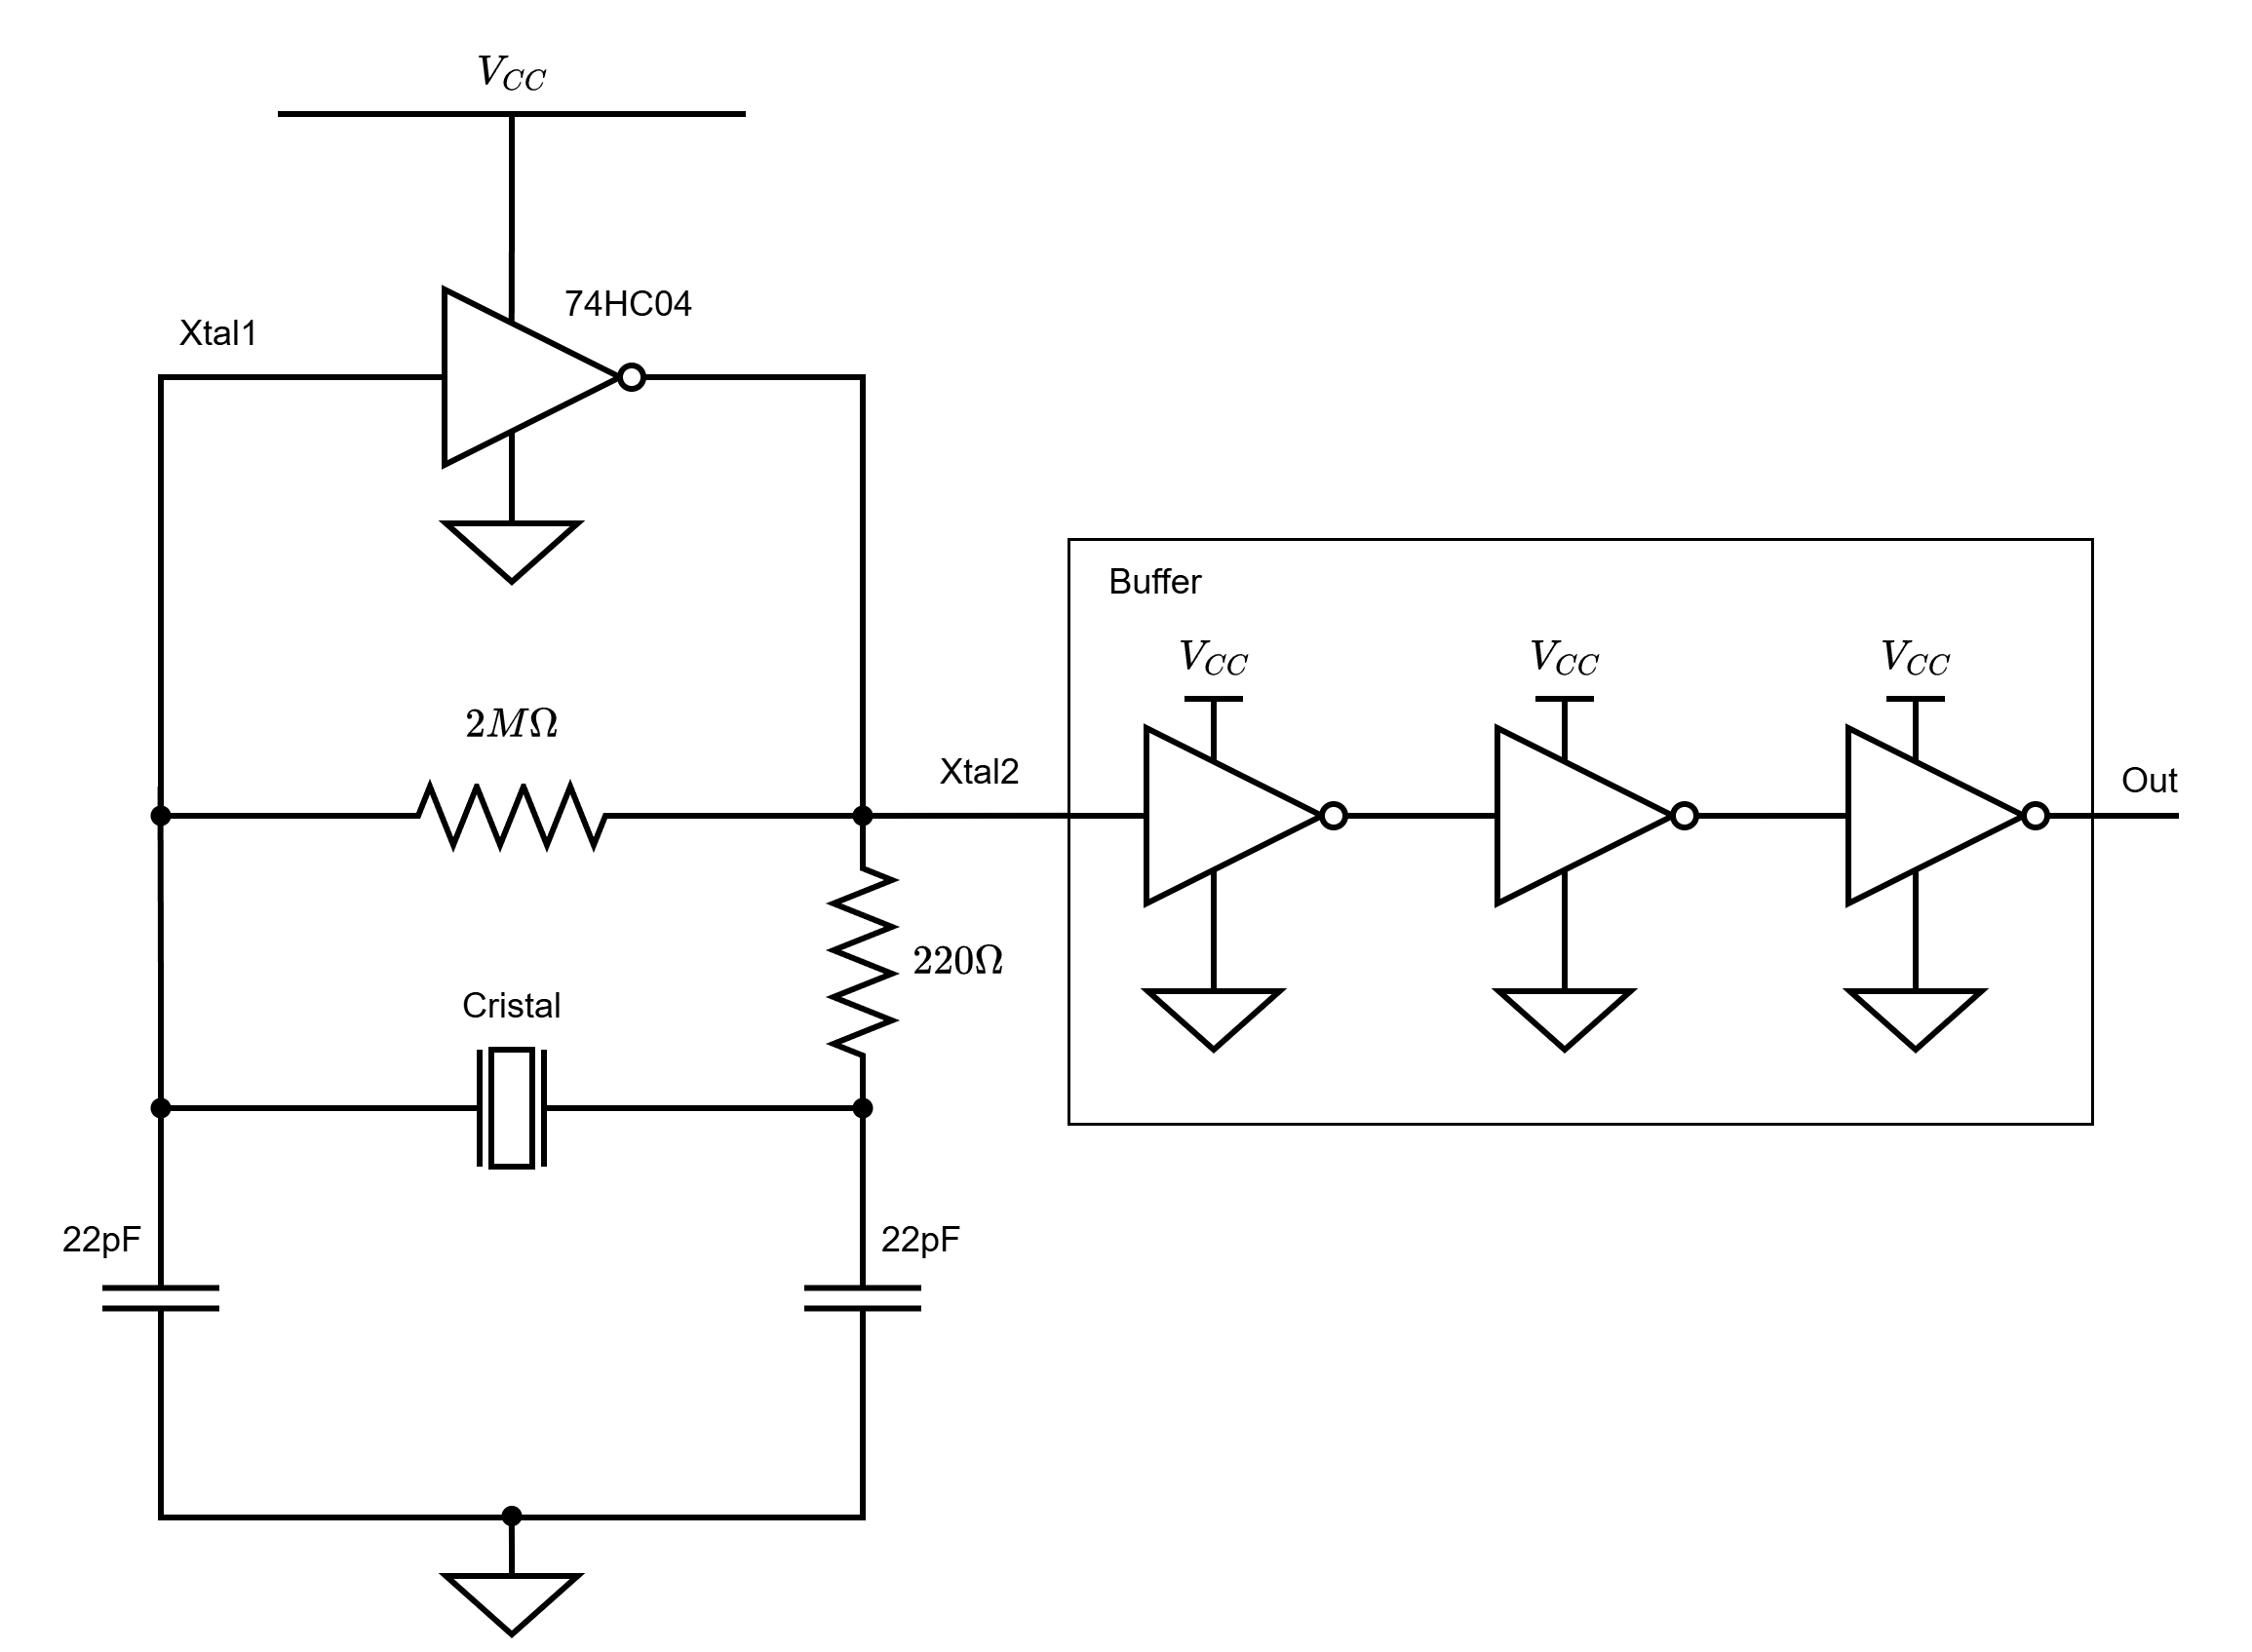
\includegraphics[width=0.90\textwidth]{../Gráficos/Oscilador/oscilador_con_buffer.png}
    \caption{Circuito oscilador implementado mediante un inversor 74HC04 y etapa de \textit{buffer} para la adquisición de la frecuencia de oscilación del cristal de cuarzo.}
    \label{fig:oscilador_qcm}
\end{figure}

El cristal de cuarzo constituye el elemento resonante del circuito y se encuentra conectado entre los nodos de entrada y realimentación del inversor. Los capacitores de $22\,\mathrm{pF}$ conectados a masa proporcionan la carga capacitiva necesaria para establecer las condiciones de oscilación y contribuyen a determinar la frecuencia de operación del conjunto.

La resistencia de $2\,\mathrm{M\Omega}$ proporciona una realimentación en continua entre la salida y la entrada del inversor. Su función es establecer un punto de operación adecuado, llevando la entrada del inversor hacia su región de transición y permitiendo que pequeñas perturbaciones presentes durante el encendido puedan ser amplificadas hasta establecer una oscilación sostenida.

Adicionalmente, se incorpora una resistencia de $220\,\Omega$ en serie con el cristal. Esta resistencia permite limitar la corriente de excitación y reducir la potencia disipada sobre el resonador, evitando una sobreexcitación que podría afectar su estabilidad y comportamiento.

\subsection{Etapa de \textit{buffer}}
\label{subsec:buffer}

La señal obtenida directamente del oscilador puede verse afectada por la impedancia de los circuitos conectados posteriormente para realizar su medición. Por este motivo, se incorporó una etapa de aislamiento o \textit{buffer} formada por tres inversores adicionales del circuito integrado 74HC04.

Esta etapa permite desacoplar el oscilador del sistema de adquisición, reduciendo la influencia que la carga de las etapas posteriores podría ejercer sobre las condiciones de oscilación del cristal. Al mismo tiempo, los inversores sucesivos regeneran la señal y proporcionan a la salida niveles lógicos adecuados para su posterior procesamiento digital.

La utilización de un número impar de inversores en la etapa de \textit{buffer} produce una inversión lógica adicional de la señal, aspecto que no resulta relevante para la aplicación desarrollada, dado que la variable de interés es la frecuencia de oscilación y no su fase. La señal obtenida a la salida de esta etapa es posteriormente utilizada como entrada del sistema encargado de realizar el conteo de pulsos y la estimación de la frecuencia del cristal.



\end{document}